
\documentclass[letterpaper, reqno,11pt]{article}
\usepackage[margin=1.0in]{geometry}
\usepackage{color,latexsym,amsmath,amssymb}
\usepackage{fancyhdr}
\usepackage{amsthm}
\usepackage{mathtools}
\usepackage{tikz}
\usepackage{float}
\usepackage{centernot}
\usepackage{subcaption}
\usepackage{extarrows}

\newcommand{\RR}{\mathbb{R}}
\newcommand{\CC}{\mathbb{C}}
\newcommand{\ZZ}{\mathbb{Z}}
\newcommand{\QQ}{\mathbb{Q}}
\newcommand{\NN}{\mathbb{N}}
\pagestyle{fancy}
\lhead{Math 321 Lecture 2}
\rhead{Yuchong Pan}
\begin{document}
\pagenumbering{arabic}
\title{Math 321 Lecture 2}
\author{Yuchong Pan}
\date{January 4, 2019}
\newtheorem{thm}{Theorem}
\newtheorem{defn}{Definition}
\newtheorem{exs}{Exercise}
\newtheorem{remark}{Remark}
\newtheorem{claim}{Claim}
\maketitle
%

\section{Pointwise and Uniform Convergence}

\subsection{Examples of Pointwise and Uniform Convergence (Cont'd)}

\begin{enumerate}
\item
  Last time we checked
  \begin{enumerate}
  \item $g_n \longrightarrow 0$ pointwise on $[0, 1]$;
  \item $g_n \centernot\longrightarrow 0$ uniformly on $[0, 1]$ (neither on $(0, 1)$);
  \item $\int_0^1 g_n(x) dx = 1 \centernot\longrightarrow \int_0^1 0dx = 0$.
  \end{enumerate}

  \begin{figure}[H]
    \centering
    \begin{tikzpicture}
      \draw[->] (-0.5, 0) -- (5, 0) node[right] {$x$};
      \draw[->] (0, -0.5) -- (0, 4) node[above] {$y$};
      \draw[domain=0:1.5, smooth, variable=\x, blue, thick] plot ({\x}, {2*\x});
      \draw[domain=1.5:3, smooth, variable=\x, blue, thick] plot ({\x}, {6-2*\x});
      \draw[domain=3:4.5, smooth, variable=\x, blue, thick] plot ({\x}, {0});
      \draw[fill=black] (1.5, 0) circle (1pt) node[below] {$\frac{1}{2n}$};
      \draw[fill=black] (3, 0) circle (1pt) node[below] {$\frac{1}{n}$};
      \draw[fill=black] (4.5, 0) circle (1pt) node[below] {$1$};
      \draw[fill=black] (0, 3) circle (1pt) node[left] {$2n$};
      \node at (3, 1.5) {$g_n(x)$};
    \end{tikzpicture}
  \end{figure}

  Similar sequences of functions:
  \begin{figure}[H]
    \centering
    \begin{subfigure}{0.4\textwidth}
      \begin{tikzpicture}
        \draw[->] (-0.5, 0) -- (5, 0) node[right] {$x$};
        \draw[->] (0, -0.5) -- (0, 4) node[above] {$y$};
        \draw[domain=0:1.5, smooth, variable=\x, blue, thick] plot ({\x}, {2*\x});
        \draw[domain=1.5:3, smooth, variable=\x, blue, thick] plot ({\x}, {6-2*\x});
        \draw[domain=3:4.5, smooth, variable=\x, blue, thick] plot ({\x}, {0});
        \draw[fill=black] (1.5, 0) circle (1pt) node[below] {$\frac{1}{2n}$};
        \draw[fill=black] (3, 0) circle (1pt) node[below] {$\frac{1}{n}$};
        \draw[fill=black] (4.5, 0) circle (1pt) node[below] {$1$};
        \draw[fill=black] (0, 3) circle (1pt) node[left] {$1$};
        \node at (3, 1.5) {$h_n(x)$};
      \end{tikzpicture}
      \subcaption{$h_n \centernot\longrightarrow 0$ uniformly on $[0, 1]$}
    \end{subfigure}
    \begin{subfigure}{0.4\textwidth}
      \begin{tikzpicture}
        \draw[->] (-0.5, 0) -- (5, 0) node[right] {$x$};
        \draw[->] (0, -0.5) -- (0, 4) node[above] {$y$};
        \draw[domain=0:1.5, smooth, variable=\x, blue, thick] plot ({\x}, {\x});
        \draw[domain=1.5:3, smooth, variable=\x, blue, thick] plot ({\x}, {3-\x});
        \draw[domain=3:4.5, smooth, variable=\x, blue, thick] plot ({\x}, {0});
        \draw[fill=black] (1.5, 0) circle (1pt) node[below] {$\frac{1}{2n}$};
        \draw[fill=black] (3, 0) circle (1pt) node[below] {$\frac{1}{n}$};
        \draw[fill=black] (4.5, 0) circle (1pt) node[below] {$1$};
        \draw[fill=black] (0, 1.5) circle (1pt) node[left] {$\frac{1}{2n}$};
        \node at (3, 1.5) {$f_n(x)$};
      \end{tikzpicture}
      \subcaption{$f_n \longrightarrow 0$ uniformly on $[0, 1]$}
    \end{subfigure}
  \end{figure}

  \begin{claim}
    \normalfont Fix any $0 < a < 1$. Then $g_n \to 0$ uniformly on $[a, 1]$.
  \end{claim}
  \begin{proof}
    Choose $N \geq 1$ integer so that $\frac{1}{n} < a$ for all $n \geq N$.
    
    \begin{figure}[H]
      \centering
      \begin{tikzpicture}
        \draw[->] (-0.5, 0) -- (4.5, 0);
        \draw[domain=0:1, smooth, variable=\x, blue, thick] plot ({\x}, {2*\x});
        \draw[domain=1:2, smooth, variable=\x, blue, thick] plot ({\x}, {4-2*\x});
        \draw[domain=2:4, smooth, variable=\x, blue, thick] plot ({\x}, {0});
        \draw[domain=3:4, smooth, variable=\x, red, thick, dotted] plot ({\x}, {0});
        \draw[fill=black] (0, 0) circle (1pt) node[below] {$0$};
        \draw[fill=black] (2, 0) circle (1pt) node[below] {$\frac{1}{n}$};
        \draw[fill=black] (3, 0) circle (1pt) node[below] {$a$};
        \draw[fill=black] (4, 0) circle (1pt) node[below] {$1$};
      \end{tikzpicture}
    \end{figure}

    Then $g_n(x) = 0$ for all $x \in [a, 1]$. Thus,
    $$ \sup_{x \in [a, 1]} |g_n(x)| = 0 \xrightarrow{n \to \infty} 0. $$
  \end{proof}
\item $h_n(x) = \frac{x^{n + 1}}{n + 1}, x \in [0, 1]$.
  \begin{enumerate}
  \item $|h_n(x) = \frac{x^{n + 1}}{n + 1} \leq \frac{1}{n} \xrightarrow{\text{uniformly}} 0$ as $n \to \infty$. Thus,
    $$ \sup_{x \in [0, 1]} |h_n(x)| = \frac{1}{n + 1} \xrightarrow{n \to \infty} 0 = h(x). $$
  \item
    $$ \int_0^1 h_n(x) dx = \int_0^1 \frac{x^{n + 1}}{n + 1} dx = \frac{1}{n + 1} \left[\frac{x^{n + 2}}{n + 2}\right]_{x = 0}^{x = 1} = \frac{1}{(n + 1)(n + 2)} \xrightarrow{n \to \infty} 0 = \int_0^1 0dx = \int_0^1 h(x) dx. $$
  \item
    $$ h_n'(x) = k_n(x) = x^n \xrightarrow[n \to \infty]{\text{pointwise}} k(x) = \left\{
    \begin{array}{ll}
      0, & x \neq 1, \\
      1, & x = 1,
    \end{array}
    \right., x \in [0, 1]. $$

    \begin{claim}
      \normalfont $k_n \centernot\longrightarrow k$ uniformly.
    \end{claim}
    \begin{proof}
      Note that
      $$ \sup_{x \in [0, 1]} |k_n(x) - k(x)| \geq \left|k_n\left(1 - \frac{1}{n}\right) - k\left(1 - \frac{1}{n}\right)\right| = \left(1 - \frac{1}{n}\right)^n \to \frac{1}{e} \neq 0. $$
      Therefore, $\sup_{x \in [0, 1]} |k_n(x) - k(x)| \geq \frac{1}{e}$ and hence $\centernot\longrightarrow 0$, proving the claim.
    \end{proof}

    \begin{figure}[H]
      \centering
      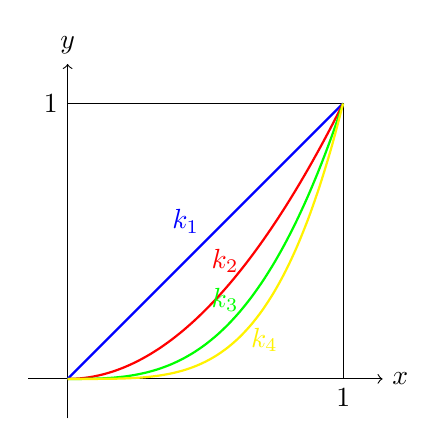
\begin{tikzpicture}
        \draw[->] (-0.5, 0) -- (4, 0) node[right] {$x$};
        \draw[->] (0, -0.5) -- (0, 4) node[above] {$y$};
        \draw (0, 0) -- (3.5, 0) -- (3.5, 3.5) -- (0, 3.5) -- (0, 0);
        \draw[scale=3.5, domain=0:1, smooth, variable=\x, blue, thick] plot ({\x}, {\x});
        \draw[scale=3.5, domain=0:1, smooth, variable=\x, red, thick] plot ({\x}, {\x^2});
        \draw[scale=3.5, domain=0:1, smooth, variable=\x, green, thick] plot ({\x}, {\x^3});
        \draw[scale=3.5, domain=0:1, smooth, variable=\x, yellow, thick] plot ({\x}, {\x^4});
        \draw[fill=black] (3.5, 0) node[below] {$1$};
        \draw[fill=black] (0, 3.5) node[left] {$1$};
        \node at (1.5, 2) [blue] {$k_1$};
        \node at (2, 1.5) [red] {$k_2$};
        \node at (2, 1) [green] {$k_3$};
        \node at (2.5, 0.5) [yellow] {$k_4$};
      \end{tikzpicture}
    \end{figure}
  \end{enumerate}
\end{enumerate}

\subsection{Theorems}

\begin{thm} \label{thm:1}
  \normalfont Let $f_n, f : (X, d) \to (Y, \rho)$. Assume
  \begin{enumerate}
  \item $f_n$ is continuous for every $n \geq 1$;
  \item $f_n \to f$ uniformly on $X$. \label{assum:2}
  \end{enumerate}
  Then, $f$ is continuous.
\end{thm}

\begin{thm} \label{thm:2}
  \normalfont Let $f_n \in C[a, b]$; i.e., $f_n : [a, b] \xrightarrow{\text{continuous}} \RR$. Assume $f_n \xrightarrow{n \to \infty} f$ uniformly on $[a, b]$. (Hence, $f \in C[a, b]$ by Theorem 1.) Then,
  $$ \int_a^b f_n(x) dx \xrightarrow{n \to \infty} \int_a^b f(x) dx. $$
\end{thm}

\begin{remark}
  \normalfont Example 1 shows that ``uniform convergence'' is necessary.
\end{remark}

\begin{remark}
  \normalfont Both theorems have a point in common; they involve {\bf interchanging limits}.
  \begin{enumerate}
  \item Theorem \ref{thm:1}:
    \begin{align*}
      & \text{ $f$ is {\bf continuous} at a point $x \in X$} \\
      \Leftrightarrow & \text{ for every sequence $\{ x_k \} \subseteq X$ with $x_k \to x$, we have $f(x_k) \xrightarrow{k \to \infty} f(x)$} \\
      \Leftrightarrow & \lim_{k \to \infty} f(x_k) = f(x) \\
      \Leftrightarrow & \lim_{k \to \infty} \underbrace{\lim_{n \to \infty} f_n(x_k)}_{(\ref{assum:2})} = \lim_{n \to \infty} f_n(x) = \lim_{n \to \infty} f_n\left(\lim_{k \to \infty} x_k\right) \xlongequal{\text{$f$ is continuous}} \lim_{n \to \infty} \lim_{k \to \infty} f_n(x_k).
    \end{align*}
  \item Theorem \ref{thm:2}:
    $$ \lim_{n \to \infty} \int_a^b f_n(x) dx = \int_a^b f(x) dx = \int_a^b \lim_{n \to \infty} f_n(x) dx. $$
  \end{enumerate}
\end{remark}

\begin{proof}[Proof of Theorem \ref{thm:2}]
  Since $f_n \to f$ uniformly on $[a, b]$, we know that given any $\epsilon > 0$, there exists $N \geq 1$ such that
  \begin{equation*} \label{eq:star}
    \sup_{x \in [a, b]} |f_n(x) - f(x)| < \epsilon \quad \forall n \geq N. \tag{*}
  \end{equation*}
  Thus,
  \begin{align*}
    \left|\int_a^b f_n(x) dx - \int_a^b f(x) dx\right| &= \left|\int_a^b [f_n(x) - f(x)] dx\right| \\
    &\leq \int_a^b |f_n(x) - f(x)| dx \\
    &\leq \int_a^b \left(\sup_{x \in [a, b]} |f_n(x) - f(x)|\right) dx \qquad \text{(by (\ref{eq:star}))} \\
    &< \int_a^b \epsilon dx \\
    &= \epsilon (b - a).
  \end{align*}
\end{proof}

\end{document}
